\subsection{Circle Packing}
For a different yet related concept to linkages, we focus on circle packing.  Before we establish the relation, we will cover some fundamental concepts of circle packings.  A \it{circle packing}, $P$, embedded in a plane  is a set of circles with disjoint interiors $\left\lbrace C_i \right\rbrace_{i = 1}^n $ such that for any circle $C \in \left\lbrace C_i \right\rbrace_{i = 1}^n$, $C$ is tangent to a different circle of $\left\lbrace C_i \right\rbrace_{i = 1}^n$. 

Any circle embedded in a plane has a given center point and radius.  This information of planar embedded circle packings allows us to establish the relationship to linkages with the following construction:
\begin{itemize}
\item[\rn{1}] let the centerpoints of the circle packing be a set of vertices $V$;
\item[\rn{2}] if two circles in a circle packing are tangent, we define an edge between their centerpoints.  The distance of this edge is the sum the radii of the two tangent circles.
\end{itemize}  
This construction establishes a relationship between linkages and circle packings.  It begs questioning as to whether every connected simple planar graph has a circle packing.  The question is answered in the following theorem.
\begin{thm}[Circle Packing Theorem]\label{thm2-1}
For every connected simple planar graph $G$ there is a circle packing in the
plane whose intersection graph is (isomorphic to) $G$.
\end{thm}
A proof of Theorem \ref{thm2-1} is found in chapter 7 of \cite{stephenson2005introduction}.  Theorem \ref{thm2-1} also gives us the ability to establish an equivalent definition of configuration spaces on circle packings and allows us to pose the same realizability problems found with simple planar graphs.  To narrow the focus of the types of circle packing realizabilty problems that we are interested in, we add the following restriction: all circles in a circle packing have unit radius. 

% \begin{definition}[Circle Packing]\label{def:circlePacking}
% $P$ of a planar graph $G$ is a set of of circles with disjoint
% interiors $\left\lbrace C_v \right\rbrace_{v \in G} $ such that two
% circles are tangent if and only if the corresponding vertices form an edge.
% \cite{arXiv13113363v1}
% \end{definition} 
% \begin{thm}[Circle Packing Theorem]\label{thm2-1}
% For every connected simple planar graph $G$ there is a circle packing in the
% plane whose intersection graph is (isomorphic to) $G$.
% \end{thm}
% \begin{figure}[!ht]
% \begin{center}
% 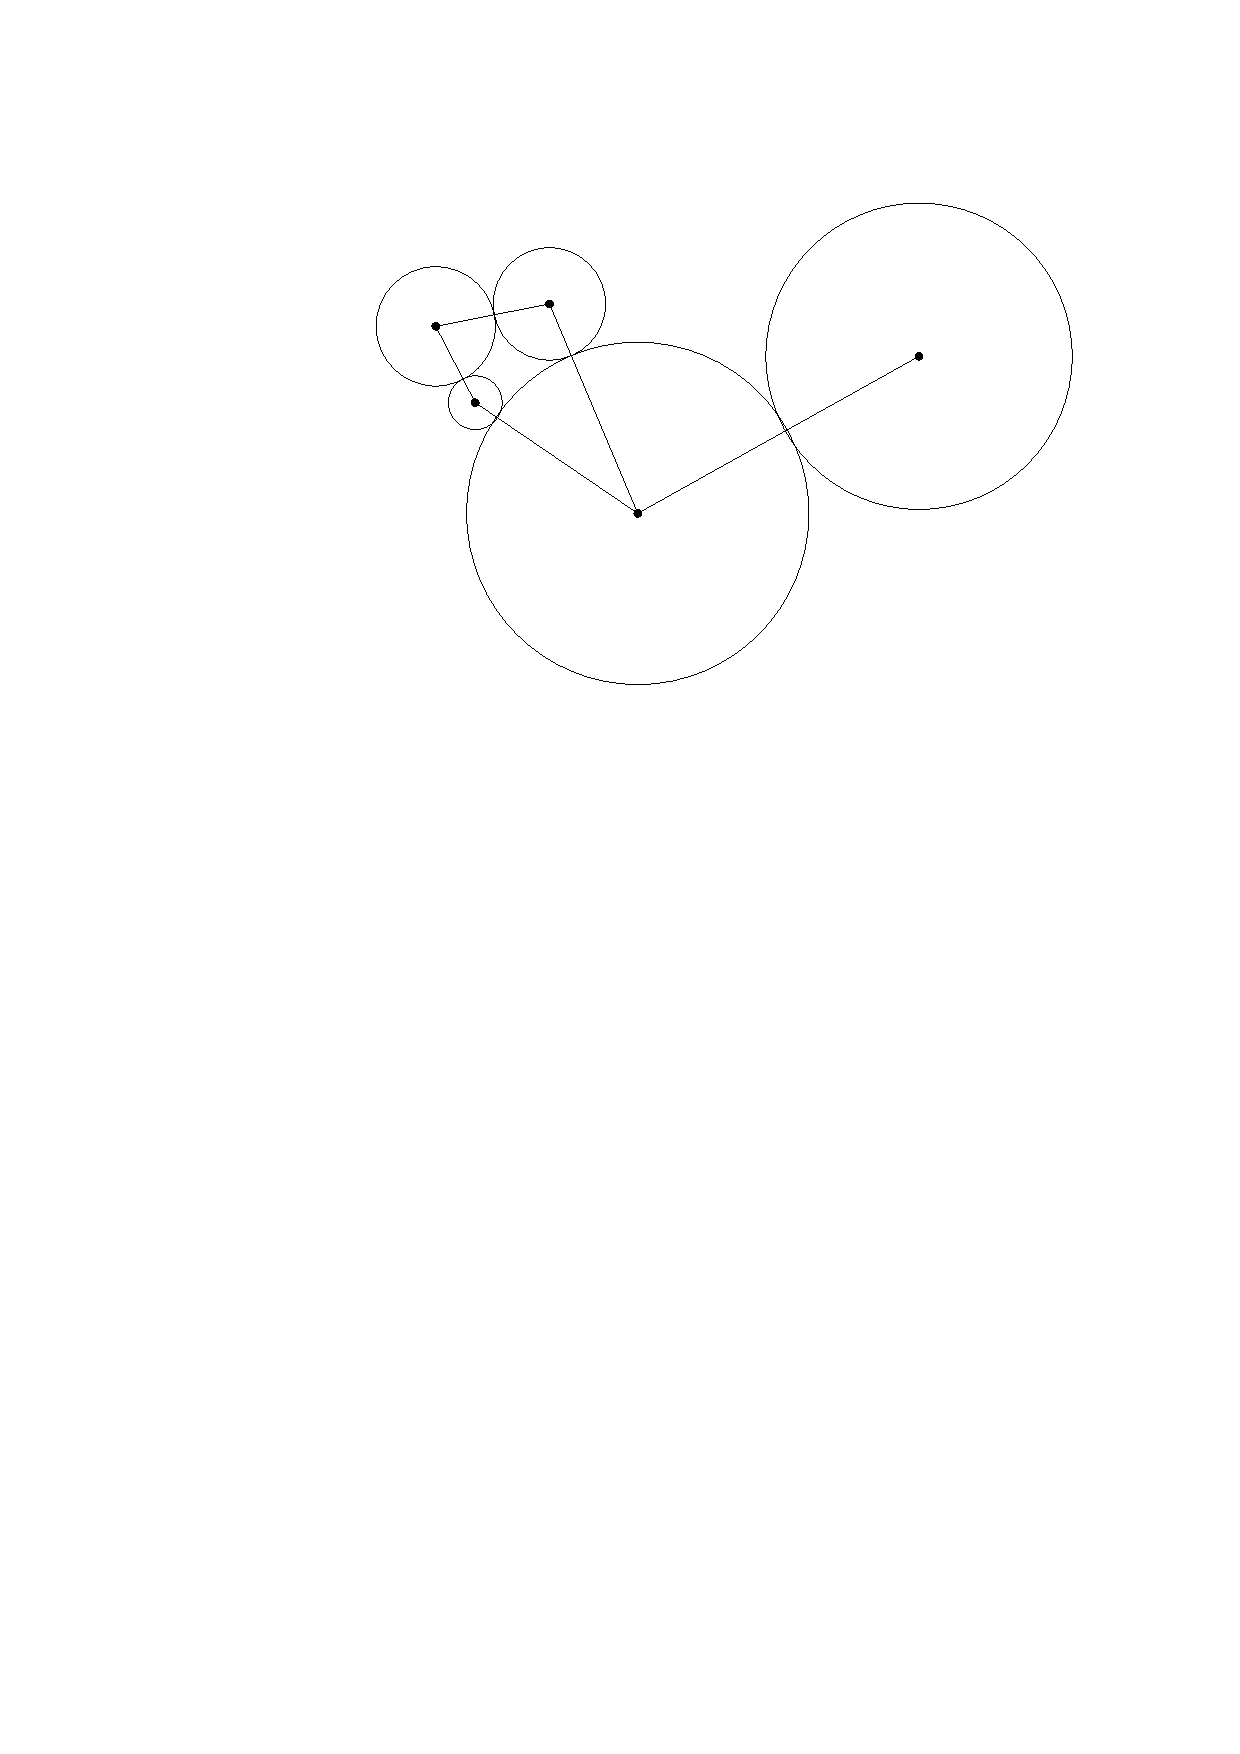
\includegraphics[scale=.5]{graphics/circlePackingTheoremExample.pdf}
% \end{center} 
% \caption{This figure is an example of a circle packing for the given simple planar graph.}
% \end{figure} 
% A proof of Theorem \ref{thm2-1} is found in \cite{stephenson2005introduction}.
% 
% \subsubsection{Circle Packings and Polygonal Linkages}
% Given a circle of radius $r$ and its center point, $(x,y)$, we establish the isomorphism  to a hexagon by
% circumscribing the vertices of the regular hexagon.
% \begin{figure}[h]
% \begin{center}
% 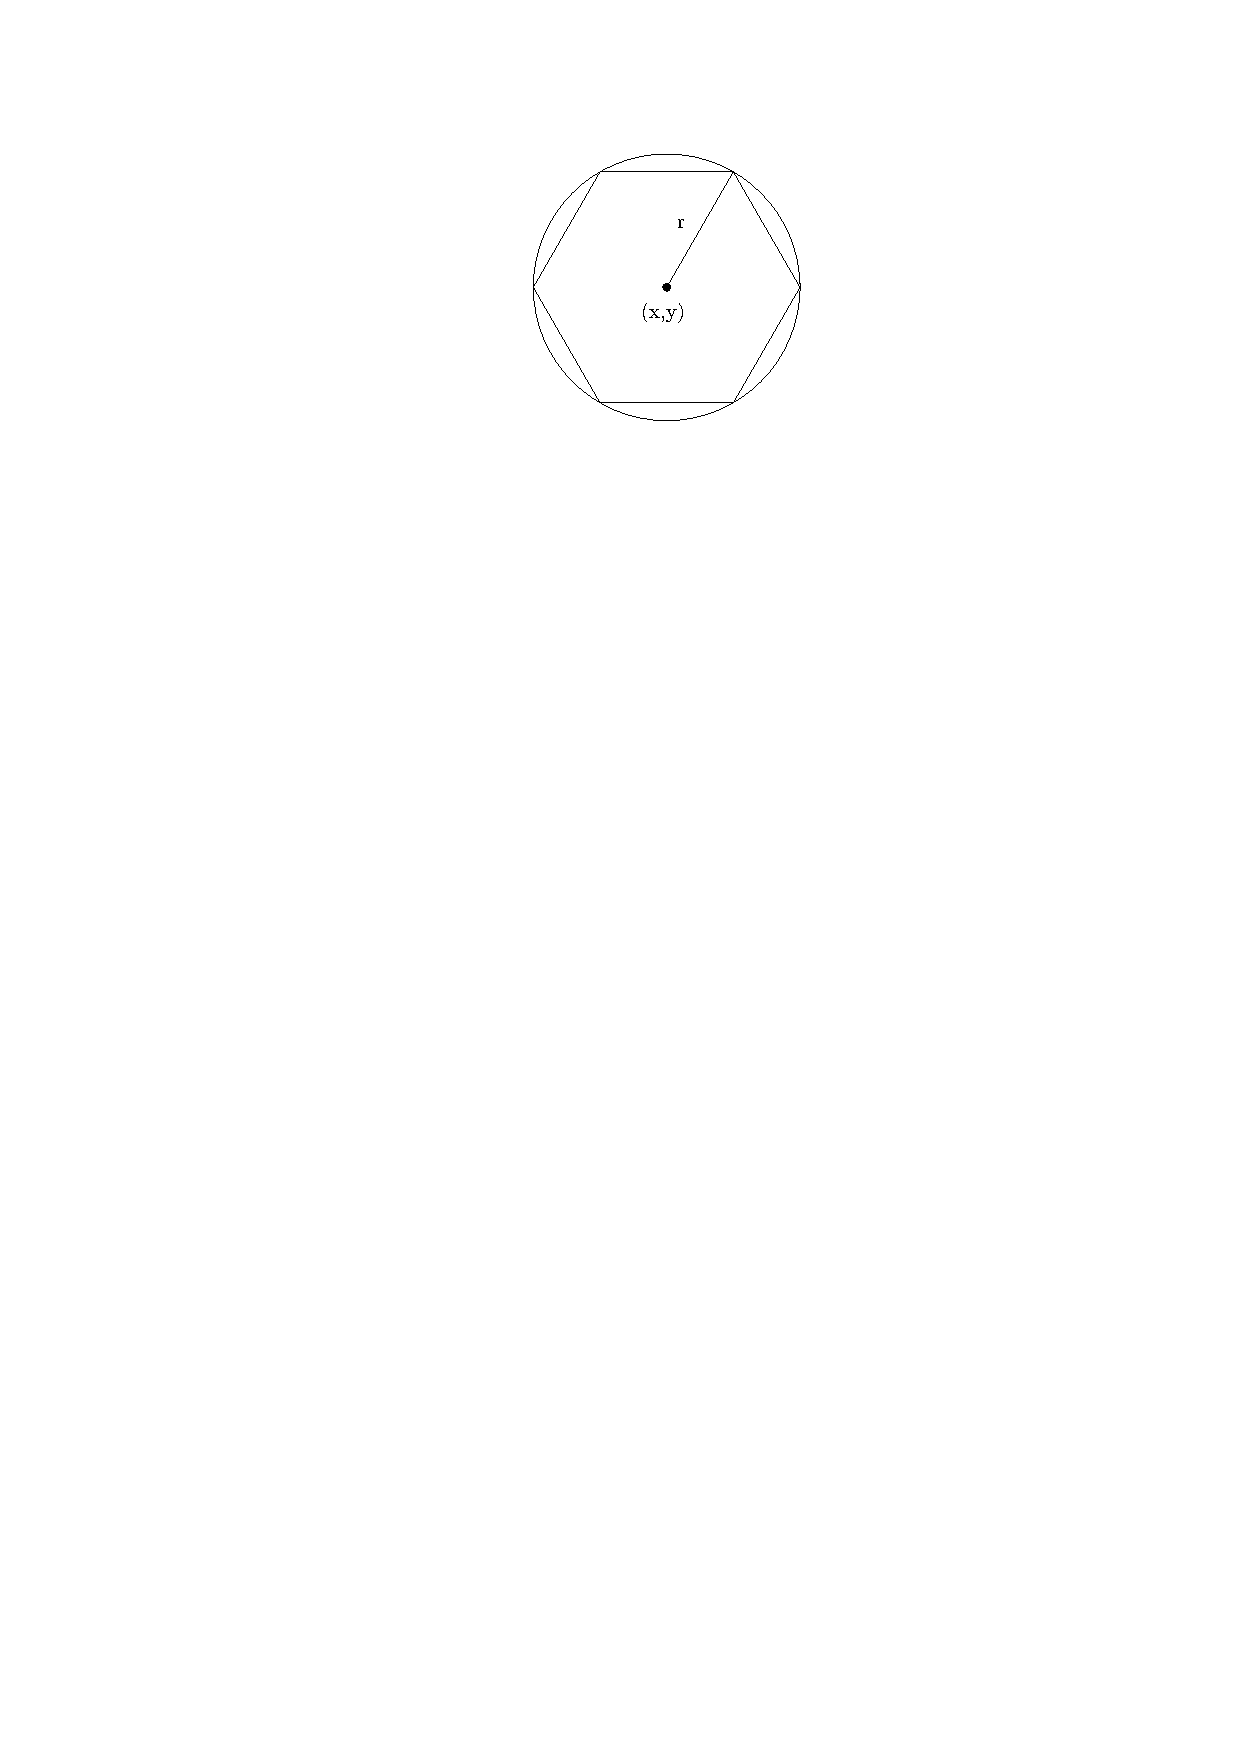
\includegraphics{graphics/circumscribedHexagon.pdf}
% \caption{A circumbscribed hexagon}
% \end{center}
% \end{figure}
\subsubsection{Hinged Polygons}
\begin{definition}[Polygonal Chain]\label{def}
A polygonal chain $P = \left( v_0, v_1, \dots, v_{n-1}\right) $ is a sequence of
consecutively joined segments (or edges) $e_i = v_i v_{i+1}$ of fixed lengths
$l_i = \left\vert e_i\right\vert $, in a plane. \cite{Biedl99lockedand}
\end{definition}
A chain is said to be closed if $v_{n-1} = v_1$, otherwise it is said to be
open. Hinged polygons have been researched for decades and related to linkage problems
\cite{Biedl99lockedand,canny1988complexity}.

Consider the locked configuration of figure \ref{figure:7hexLocked}.  We can
 configure the hexagons to be locked by placing hinged points as follows:
\begin{figure}[!ht]
\begin{center}
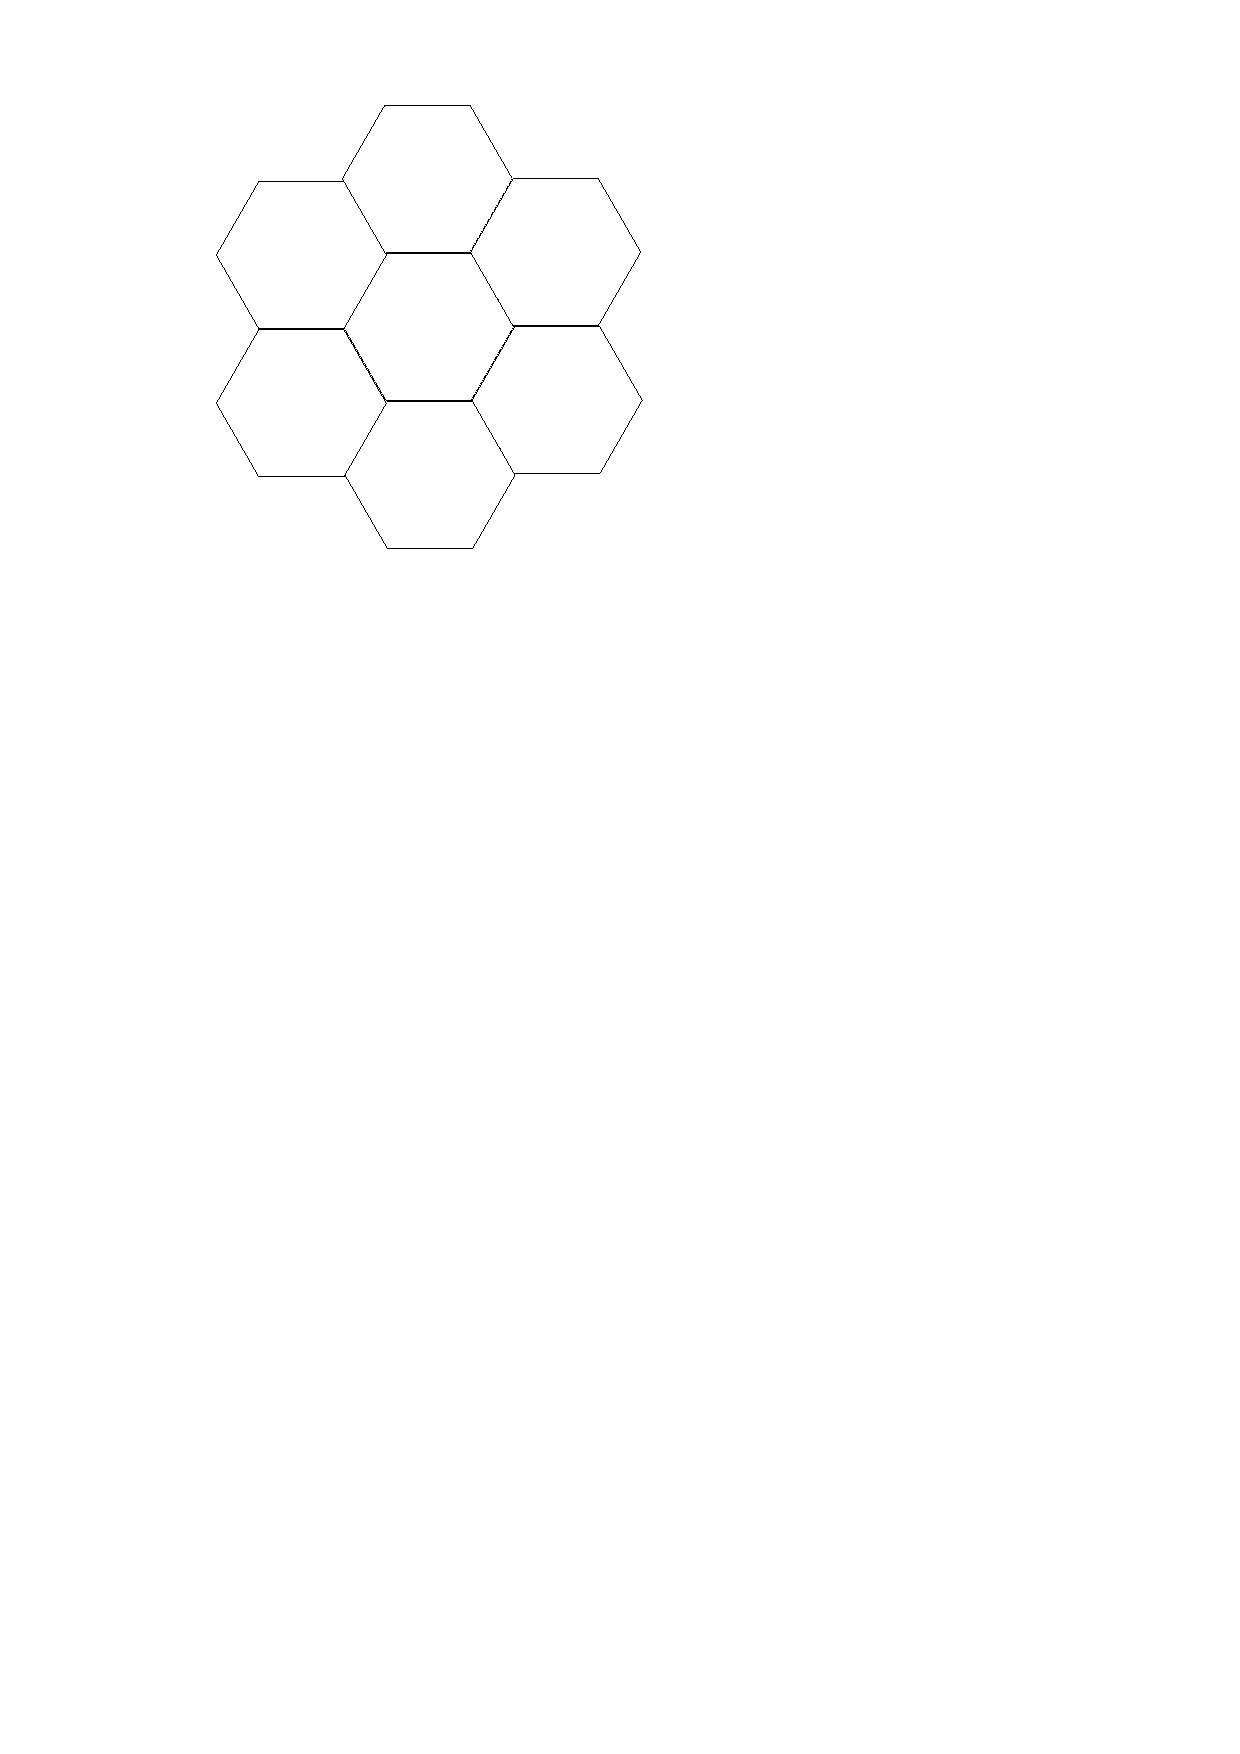
\includegraphics[scale=.33]{graphics/7hexLocked.pdf}
\caption{A locked 7 hexagonal configuration.  (needs to modify picture by
placing red points for hing points.)}
\label{figure:7hexLocked}
\end{center} 
\end{figure}

\subsubsection{Hinged Hexagons of Fixed Size}

\paragraph{The Shapes}
Figure \ref{fig:lockingShape} is a locking shape:
% \begin{figure}[h]
% \begin{center}
% 
\includegraphics{graphics/lockingShape.pdf}
% \caption{This is the shape that resides in boundary of the lattice.}
% \label{fig:lockingShape}
% \end{center}
% \end{figure}
\begin{figure}[h]
\begin{center}
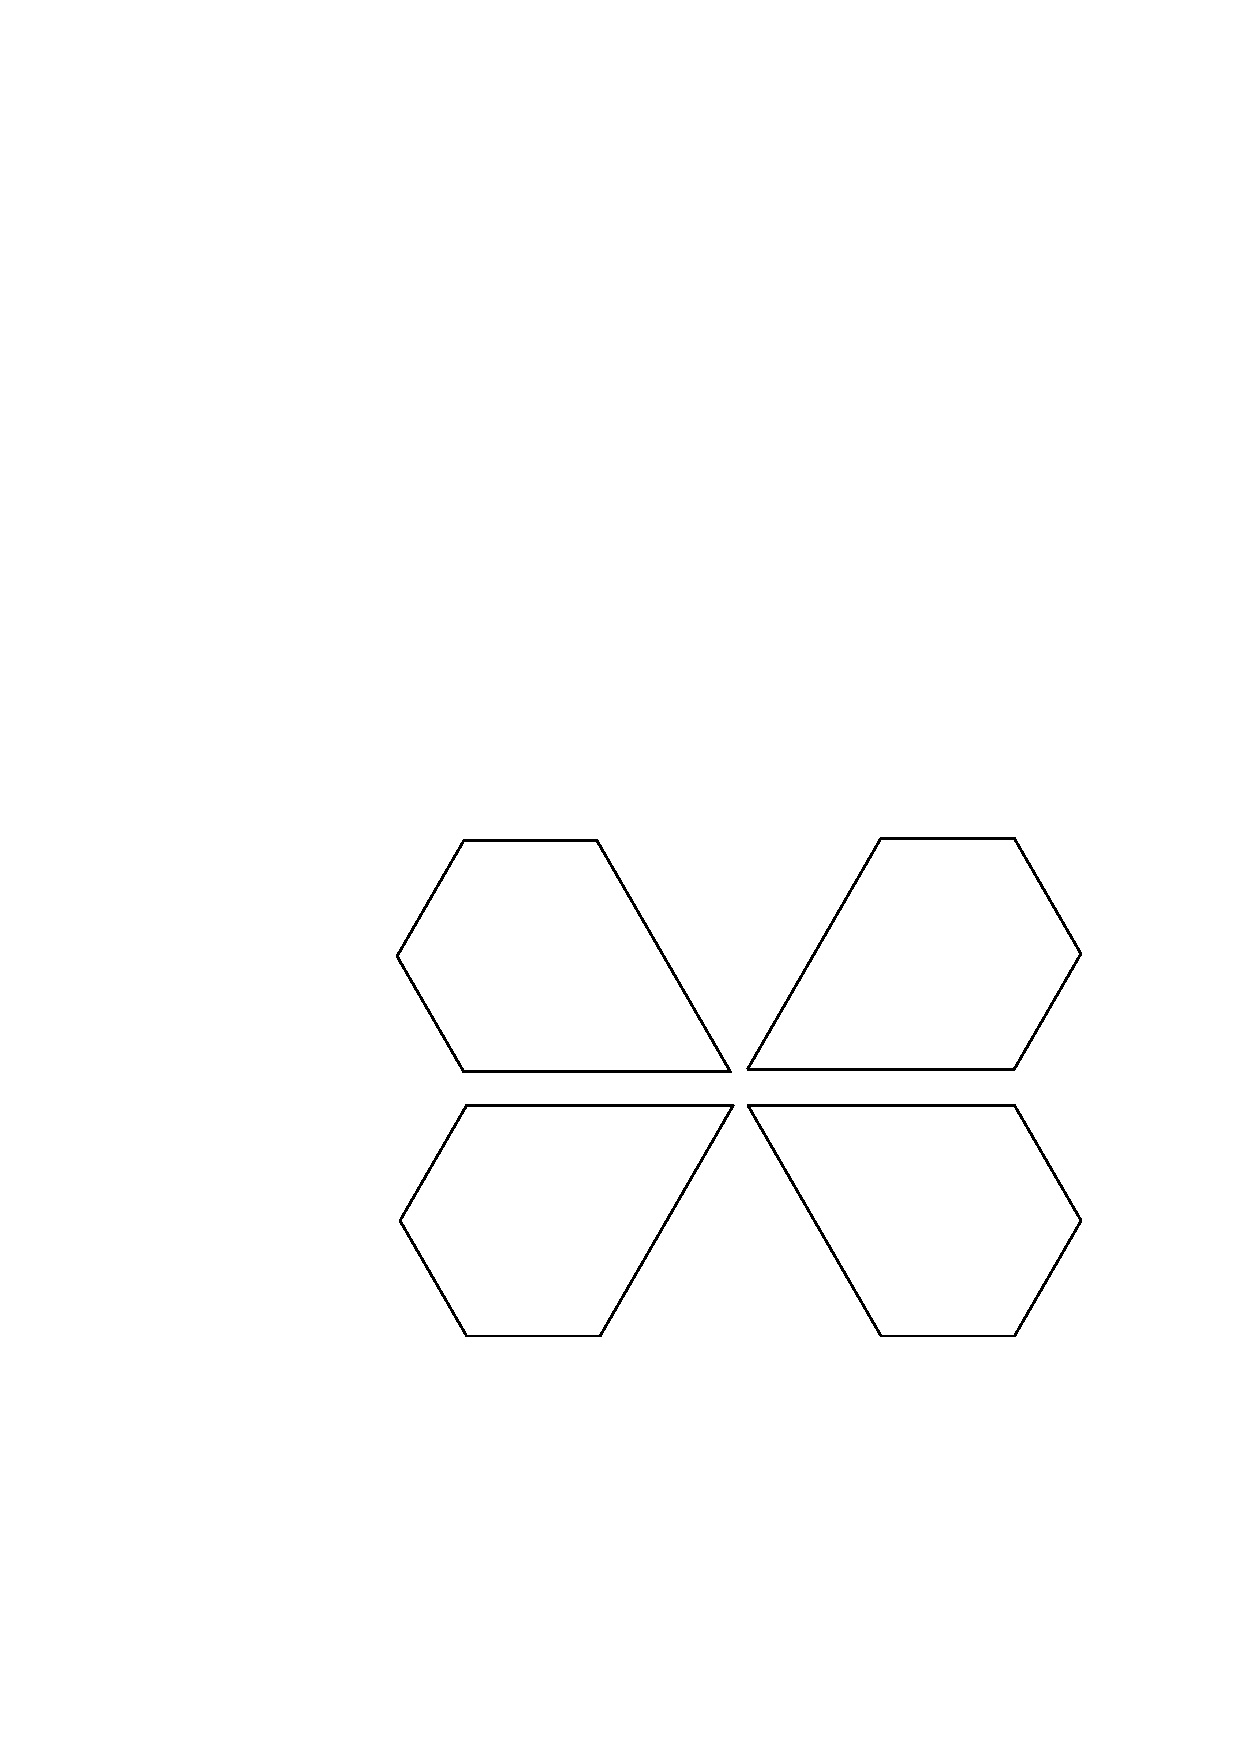
\includegraphics[scale=.33]{graphics/shapeInChannel.pdf}
\end{center} 
\caption{A locking shape in the lattice boundary's channel.}
\label{fig:lockingShape}
\end{figure}
Figure \ref{fig:lockingShape} shall reside in the boundary of a lattice and have
a hinge point at one vertex where the locking shape and boundary meet.

\paragraph{Junctions}
We define junctions to be the point three hexagons meet in a hexagonal lattice,
e.g. Figure \ref{fig:lattice}.
%Radius of regular polygons 
\newdimen\R
\R=4.5cm
\begin{figure}[h] 
\begin{center}
\begin{tikzpicture}
\begin{scope}
\filldraw[pattern=hexagons]  (0:\R) \foreach \x in {60,120,...,359} {
                -- (\x:\R)
            }-- cycle (90:\R);
\end{scope}
\end{tikzpicture}
\caption{A portion of a hexagonal lattice.}
\label{fig:lattice}
\end{center}
\end{figure}
\newpage
\paragraph{Central Scaling}
\paragraph{Junctions in Conjunctive Normal Form}
Explain the configurations we're interested in.
